\documentclass[10pt]{beamer}

\usepackage[english]{babel}
\usepackage[utf8]{inputenc}
\usepackage{amsmath}
\usepackage{amssymb}
\usepackage{amsthm}
\usepackage[all]{xy}
\usepackage{graphicx}
\usepackage{tikz}
\usetikzlibrary{arrows,shapes,automata}
\usepackage[style=beamer,doi=false,isbn=false,eprint=false,maxnames=10]{biblatex}
\bibliography{../defeo}
\usepackage{mysymbols}
\usepackage{textcomp}
\usepackage{listings}
\lstset{
  language=haskell,
  upquote=true,
  basicstyle=\ttfamily,          % print whole listing in typewriter
  keywordstyle=\color{blue}\bfseries, % bold blue keywords
  %identifierstyle=,           % nothing happens
  commentstyle=\color{green}, % green comments
  stringstyle=\color{red},      % typewriter type for strings
  showstringspaces=false     % no special string spaces
}


\usepackage[amssymb,amsfonts]{concmath}
\renewcommand{\sfdefault}{uop}
\mode<presentation>{%
  \usetheme{Boadilla}
  \usefonttheme[onlymath]{serif}
  \usecolortheme[rgb={0.56,0.3,0}]{structure}
  \setbeamercolor{alerted text}{fg=blue}
}
\renewcommand{\emph}[1]{{\usebeamercolor[fg]{structure}#1}}

\title[Explicit isogenies and related topics]{On the efficient computation of explicit isogenies and related topics}
\author{Luca~De~Feo}
\institute[IRMAR]{IRMAR, Université de Rennes 1}
\date[Versailles, May 12, 2011]{May 12, 2011\\Séminaire Crypto, PRISM, UVSQ}

\AtBeginSection[]
{
  \begin{frame}<beamer>
    \frametitle{Outline}
    \tableofcontents[currentsection]
  \end{frame}
}


\begin{document}

\begin{frame}
  \titlepage
\end{frame}

%%

\begin{frame}
  \frametitle{The last SEA record}

  \begin{block}{From Andrew Sutherland's web page: \url{http://math.mit.edu/~drew/SEArecords.html}}
    July 7, 2010
    
    The number of points on the elliptic curve E defined by the equation
    
    \[y^2 = x^3 + 2718281828x + 3141592653,\]
    
    modulo the prime $p=16219299585*2^{16612}-1$ is $p+1-t$, where the
    Frobenius trace $t$ is [a 2500-digit integer].
  \end{block}

  \begin{block}{}
    \centering
    \begin{tabular}{l r}
      \emph{Task} & \emph{Total CPU time}\\
      \hline
      Compute $\Phi^f_n(X,j(E)) \bmod p$ & 32 days\\
      Compute $X^p \bmod \Phi^f_n(X,j(E))$ & 995 days\\
      Construct the Elkies kernel polynomial $h_n(X)$ & 3 days\\
      Compute $Y^p$ mod $h_n$ and derive $X^p$ mod $h_n$ & 326 days\\
      Find the Frobenius eigenvalue $\lambda_n$ using BSGS & 22 days 
    \end{tabular}
  \end{block}
\end{frame}

%%

\begin{frame}
  \frametitle{The last SEA record}

  What's behind the record?
  \begin{itemize}
    \setlength{\itemsep}{\baselineskip}
  \item (Mildly) parallel computation;
  \item A lot of number theory to find smaller modular polynomials
    \parencite{enge+sutherland10};
  \item A space efficient, CRT algorithm to compute $\Phi^f_n \bmod p$
    and derived
    quantities \parencite{fouquet+gaudry+harley00,sutherland10:modpol};
  \item Fast integer arithmetic using GMP;
  \item Highly optimized polynomial arithmetic over finite fields
    (V. Shoup's NTL library, \cite{gaudry+morain06}, \dots);
  \item A cache friendly truncated FFT algorithm \parencite{harvey+roche10}.
  \end{itemize}

\end{frame}

%% 
%%

\section{Explicit isogenies}

\begin{frame}
  \frametitle{Elliptic curves}

  \begin{itemize}
  \item Curves of genus $1$,
  \item Abelian varieties of dimension $1$.
  \end{itemize}
  
  \begin{block}{(Short) Weierstrass form}
    Assuming $p\ne2,3$
    {\large
      \begin{equation*}
        E\;:\;y^2 = x^3 + ax + b\qquad\text{with $a,b\in\K$.}
      \end{equation*}
    }
    \begin{itemize}
    \item discriminant: \alert{$\Delta_E = -16(4a^3 + 27b^2) \ne 0$} (the curve is non-singular),
    \item $j$-invariant: \alert{$j_E=\frac{-1728(4a^3)}{\Delta_E}$}
      ($j_E=j_{E'} \Leftrightarrow E\isom E'$ over $\clot{\K}$),
    \item invariant differential: \alert{$\omega_E= \diff x/(2y)$} (invariant under translation).
    \end{itemize}
  \end{block}
\end{frame}

%%

%%

\begin{frame}
  \frametitle{Group law and scalar multiplication}
  
  \begin{columns}
    \begin{column}{0.3\textwidth}
      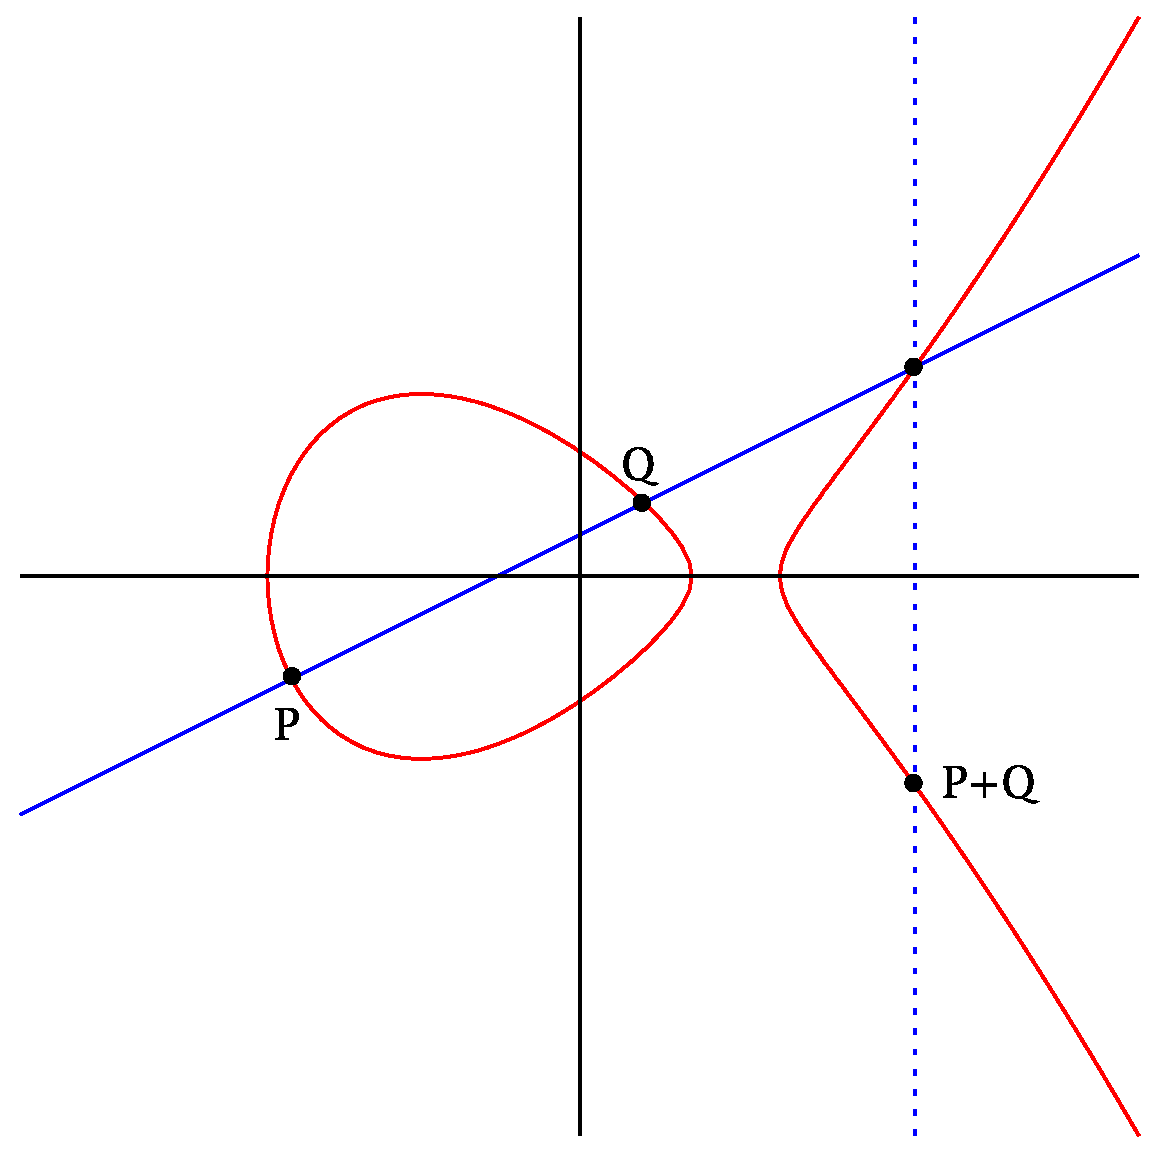
\includegraphics[width=\textwidth]{../isogeny/ec-add.pdf}
    \end{column}
    \begin{column}{0.55\textwidth}
      {\large\emph{\[y^2 = x^3 + ax + b\]}}
      \begin{gather*}
        P = (x_0, y_0), Q = (x_1, y_1)\\
        \lambda = \frac{y_1 - y_0}{x_1 - x_0}\\
        P+Q = (\lambda^2 - x_0 - x_1, (x_0 - x_2)\lambda - y_0)
      \end{gather*}
    \end{column}
  \end{columns}

  {\large
    \begin{description}
    \item[\emph{Multiplication:}] $[m]P = \overbrace{P + P + \cdots + P}^{\text{$m$ times}}$
    \item[\emph{$m$-torsion:}] $E[m] = \{P\in E(\clot{\K}) | [m]P=\0\} \isom (\Z/m\Z)^2$
    \end{description}}
  
  \[[m](x,y) = \left(\frac{\psi_m(x,y)}{\phi_m^2(x,y)}, \frac{\omega_m(x,y)}{\phi_m^3(x,y)}\right)\]
  
  \emph{Division polynomials:} $\phi_m$ can be computed with $O(\log
  m)$ polynomial multiplications, $\deg\phi_m=O(m^2)$.
\end{frame}

%%

% \begin{frame}
%   \frametitle{Elliptic curves over $\C$}

%   \begin{center}
%     Nice picture goes here
%   \end{center}
  
%   \begin{block}{Weierstrass $\wp$-function}
%     \[\wp(z) = \frac{1}{z^2} +
%     \sum_{\omega\in\Lambda\backslash\{0\}}\frac{1}{(z-\omega)^2}-\frac{1}{\omega^2}\]

%     Satisfies
%     \begin{equation*}
%       {\wp'}^2 = 4\wp^3 - 60G_4\wp - 140G_6.
%     \end{equation*}

%     We have an isomorphism:
%     \begin{equation*}
%       \begin{aligned}
%         \C/\Lambda &\to E(\C)\\
%         z &\mapsto\left(\wp(z),\wp'(z)\right).
%       \end{aligned}
%     \end{equation*}
%   \end{block}
% \end{frame}

%%

\begin{frame}
  \frametitle{Isogenies}
  
  \vspace{-5mm}

  {\large \[\xymatrix{E\ar[d]_{[m]}\ar[r]^{\I} & E'\ar[dl]^{\hat{\I}}\\E}\]} 
  \emph{\textbf{(Separable) isogeny:}} (separable)
  non-constant rational morphism preserving the identity.
  
  \begin{block}{Properties}
    \begin{itemize}
    \item Isogeny = rational map $\;+\;$ group morphism;
    \item Finite kernel, surjective (in $\clot{\K}$);
    \item \emph{Dual isogeny theorem:} they factor the multiplication map into two pieces.
    \end{itemize}
  \end{block}

  \vspace{-1mm}

  \begin{block}{
	\begin{overprint}
	\onslide<1> Multiplication	
	\onslide<2> Frobenius endomorphism
	\onslide<3> Separable isogeny (short Weierstrass form)
	\end{overprint}
      }
    \begin{overprint}
      \onslide<1>
      \[\begin{aligned}
	{}[m] : E(\clot{\K}) &\rightarrow E(\clot{\K})\\
	                   P &\mapsto [m]P
      \end{aligned}\]
      $\ker\I = E[m]$.

      \onslide<2>
      \[\begin{aligned}
	\frob : E(\clot{\K}) &\rightarrow E(\clot{\K})\\
	               (x,y) &\mapsto (x^q,y^q)
      \end{aligned}\]
      $\ker\frob = \{\0\}$ (inseparable).

      \onslide<3>
      \[\quad\I(x,y) = \left(\frac{g(x)}{h(x)},
      cy\left(\frac{g(x)}{h(x)}\right)'\right)\]
      $h\;$ vanishes on the abscissas of $\;\ker\I$. \emph{$\quad\deg\I \;=\; \card{\ker\I}$}.
    \end{overprint}
  \end{block}  
\end{frame}

%%

\begin{frame}
  \frametitle{Why compute (large) isogenies over finite fields?}
  
  \begin{block}{SEA algorithm (\cite{schoof85,elkies92,atkin88})}
    \begin{description}
    \item[Hasse bound] \hfill{\large\emph{$\card{E(\F_q)}= q-t+1$}};\hfill\strut
    \item[Schoof] Compute $t$ modulo small primes
      $\ell\;\Leftrightarrow$ compute the action of $\frob_q$ on
      \emph{$E[\ell]\;\isom\;(\Z/\ell\Z)^2$};
    \item[Atkin] Determine the order of the roots of $X^2 -tX +q$ by
      factoring the $\ell$-th modular polynomial;
    \item[Elkies] Compute an $\ell$-isogeny $\I$ and the action of
      $\frob_q$ on \emph{$\ker\I\;\isom\;\Z/\ell\Z\;\subset\;E[\ell]$}.
    \end{description}
  \end{block}

  \begin{block}{Other cryptographic applications}
    \begin{itemize}
    \item Transfer DLPs between curves (\cite{gaudry+hess+smart02,smith09});
    \item Construct new cryptosystems (\cite{teske06,rostovtsev+stolbunov06});
    \item Construct hash functions (\cite{charles+lauter+goren09});
    \item Compute modular polynomials (\cite{sutherland10:modpol});
    \item Compute the endomorphism ring (\cite{kohel,bisson+sutherland11}).
    \end{itemize}
  \end{block}
\end{frame}

%%
%%

\begin{frame}
  \frametitle{Vélu's formulas}
  
  \begin{block}{Compute an isogeny with given kernel (\cite{velu71})}
    Given the kernel $H$, computes $\;\I : E\to E/H\;$ given by
    \begin{align*}
      &\I(\0_E) = \I(\0_{E/H})\text{,}\\
      &\begin{aligned}
        \I(P) = \Biggl(x(P) + \sum_{Q\in H^\ast}x(P+Q) - x(Q),
        y(P) + \sum_{Q\in H^\ast}y(P+Q) - y(Q) \Biggr) \text{.}
      \end{aligned}
    \end{align*}
  \end{block}

  \begin{block}{In practice, given $h(x)$, of degree $\ell-1$,
      vanishing on $H$}
    {\footnotesize
      \[
      y^2 = f(x)\text{,}
      \qquad
      p_1 = \sum_{Q\in H^\ast} x(Q)\text{,}
      \qquad
      \frac{g(x)}{h(x)} = \ell x - p_1 - f'(x)\frac{h'(x)}{h(x)} - 2f(x)\left(\frac{h'(x)}{h(x)}\right)'\]}
    \[\alert{\I(x,y) = \left(\frac{g(x)}{h(x)}, y\left(\frac{g(x)}{h(x)}\right)'\right)}\]
  \end{block}
\end{frame}

%%

\begin{frame}
  \frametitle{Computing the kernel of an isogeny}
  
  \begin{block}{\textbf{Goal:} Given $E, \ell$, compute $\I:E\to E'$ of degree $\ell$}
    \begin{itemize}
    \item \emph{\cite{strak73}}: First algorithm in characteristic
      $0$, using continued fractions.
    \item \emph{\cite{elkies92,elkies98}:} Find a power series
      solution to the differential equation.
    \item \emph{\cite{couveignes94}:} ($p$ small) Compute morphisms of
      formal groups, look for one that corresponds to an isogeny.
    \item \emph{\cite{lercier96}:} (only for $p=2$) solve a linear
      system.
    \item \emph{\cite{couveignes96}:} ($p$ small) Interpolate over the
      $p$-torsion, look for a polynomial that corresponds to an
      isogeny.
    \item \emph{BMSS
        algorithm \parencite{bostan+morain+salvy+schost08}:} Improve
      \cite{elkies98} to run in quasi-linear time.
    \item \emph{\cite{lercier+sirvent08}:} Lift $E$ and $E'$ in the
      $p$-adics, then apply BMSS.
    \end{itemize}
  \end{block}
\end{frame}

%%

\begin{frame}
  \frametitle{Modular polynomial}

  \begin{center}
    $\Phi_\ell(X,Y)$, the minimal polynomial over $\C$ of the modular
    function $j(\ell\tau)$
  \end{center}

  \begin{block}{Properties}
    \begin{itemize}
    \item The roots of $\Phi_\ell(X,j(E))$ are the $j$-invariants
      of the elliptic curves $\ell$-isogenous to $E$;
    \item Symmetric in $X$ and $Y$, degree $\ell+1$;
    \item Integer coefficients of size $O(\ell\log\ell)$.
    \end{itemize}
  \end{block}

  \begin{block}{Computation}
    \begin{itemize}
    \item By evaluation-interpolation over $\C$ in $\tildO(\ell^3)$  (\cite{enge09}),
    \item $\Modpol_\ell\bmod p$ in $\tildO(\ell^2\log p)$ \alert{only
        for special $p$'s},
    \item By CRT $\Modpol_\ell\bmod m$ in $\tildO(\ell^3)$ using only
      $\tildO(\ell^2\log m)$ space by CRT (\cite{sutherland10:modpol}).
    \end{itemize}
  \end{block}
\end{frame}

%%

\begin{frame}
  \frametitle{Algorithms based on the differential equation}
  
  
  \begin{block}{Normalized isogenies}
    By Vélu's formulas: $\I(x,y) = \left(\I_x(x), y\I_x'(x)\right)$,
    hence given isogenous models
    \begin{equation*}
      E \;:\; y^2 = x^3 + ax + b,\qquad
      E' \;:\; y^2 = x^3 + a'x + b
    \end{equation*}
    the isogeny verifies
    \begin{equation}
      \label{eq:1}
      \left(\alert{c}y\I_x(x)'\right)^2 = \I_x(x)^3 + a'\I_x(x) + b'.
    \end{equation}

    When \alert{$c=1$}, the isogeny is said to be \emph{normalized}.
  \end{block}

  \begin{block}{Algorithm (\cite{elkies98,bostan+morain+salvy+schost08})}
    \begin{enumerate}
    \item Find an $\ell$-isogenous $j$-invariant
      $j_{E'}$;\hfill\alert{$\tildO(\ell^3)$}
    \item Compute a \emph{normalized} model for $E'$;\hfill\alert{$\tildO(\ell^3)$}
    \item Solve the differential equation \eqref{eq:1}.\hfill\alert{$\tildO(\ell)$}
    \end{enumerate}
    Steps $1$ and $2$ can be replaced by an algorithm to evaluate
    large degree isogenies with complexity
    \alert{$O\left(L_q(1/2)\log\ell\right)$} (\cite{jao+soukharev10}).
  \end{block}
\end{frame}

%%

\begin{frame}
  \frametitle{Couveignes' algorithm (\cite{couveignes96})}
  
  \begin{center}
    \large
    Given $E, E', \ell$, compute $\I:E\to E'$
  \end{center}

  \begin{center}
    \emph{\textbf{Idea:}} Map $E[p^k]$ onto $E'[p^k]$
  \end{center}
  
  \begin{itemize}
  \item Compute the extensions $\U_i/\F_q$ such that $E[p^i]$ is
    defined over $\U_i$;
    \uncover<1-2>{\hfill\emph{\alt<1>{$\tildO(\ell^2)$}{\alert{$\tildO(\Mult(\ell))$}}}}
  \item Pick $\;k\;$ \emph{large enough} ($k\sim\log_p4\ell$);
  \item Compute $\;P$, a generator of $\;E[p^k]$;
    \uncover<1-2>{\hfill\emph{\alt<1>{$\tildO(\ell^2)$}{\alert{$\tildO(\Mult(\ell))$}}}}
  \item Compute $\;P'$, a generator of $\;E'[p^k]$;
    \uncover<1-2>{\hfill\emph{\alt<1>{$\tildO(\ell^2)$}{\alert{$\tildO(\Mult(\ell))$}}}}
  \item Compute the polynomial $\;T\;$ vanishing on $\;E[p^k]$;
    \uncover<1-2>{\hfill\emph{\alt<1>{$\tildO(\ell^2)$}{\alert{$\tildO(\Mult(\ell))$}}}}
  \item For $m\in\left(\Z/p^k\Z\right)^\ast$
    \begin{itemize}
      \normalsize
    \item Interpolate $\;A : x(P) \mapsto x([m]P')$;
      \uncover<1-2>{\hfill\emph{\alt<1>{$\tildO(\ell^2)$}{\alert{$\tildO(\Mult(\ell))$}}}}
    \item Reconstruct a rational fraction  $\;\frac{g}{h}\equiv A \bmod T$;
      \uncover<1-2>{\hfill\emph{$\tildO(\Mult(\ell))$}}
    \end{itemize}
    \alert<3>{Stop when $\frac{g}{h}$ is an isogeny.}
    \uncover<1-2>{\hfill\emph{$\ell$ times on average}}
  \end{itemize}
\end{frame}

%%

\begin{frame}
  \frametitle{How to recognize an isogeny?}

  \begin{itemize}
    \setlength{\itemsep}{\baselineskip}
  \item \emph{\textbf{Degree:}} $\frac{g}{h}\;$ with $\;\deg g=\ell$, $\;\deg h = \ell-1$;\hfill\alert{$O(1)$}
  \item \emph{\textbf{Square factor:}} $h = \prod_{Q\in H^\ast}(X-
    x(Q)) = f^2\;$ if $\ell$ odd;\hfill\emph{$\tildO(\Mult(\ell))$}
  \item \emph{\textbf{Group action:}} Test on random points: $\;\I(P+Q)=\I(P)+\I(Q)$;\hfill\emph{$O(\ell)$}
  \item \emph{\textbf{Factor of the $\ell$-division polynomial:}}
    Check $\phi_\ell=0\bmod h$.\hfill\emph{$\tildO(\Mult(\ell))$}
  \end{itemize}
\end{frame}

%%

\begin{frame}
  \frametitle{How to recognize an isogeny?}
  
  \begin{center}
    $T\;$ vanishes on $\;E[p^k]$, $A$ interpolates $x(P)\mapsto x(P')$
  \end{center}
  
  \[AU_i + TV_i = R_i  \qquad\Leftrightarrow\qquad  A\equiv \frac{R_i}{U_i} \bmod T\]
  \[\ell = 11\]
  \pause
  \begin{center}
  \begin{tabular}{c | c}
    $\deg R_i$ & $\deg U_i$ \\
    $3141592653589793238462643$ & 0 \\
    \pause
    $3141592653589793238462642$ & 1 \\
    \pause
    $3141592653589793238462641$ & $2$ \\
    \pause
    \vdots & \vdots\\
    $3141592653589793238462634$ & $9$ \\
    \pause
    \Huge\alert{$11$} & \Huge\alert{$10$}\\
    \pause
    $10$ & $3141592653589793238462633$\\
    \vdots & \vdots
  \end{tabular}
  \end{center}
\end{frame}

%%

\begin{frame}
  \frametitle{Isogenies of unknown degree}
  
  \large 

  \begin{itemize}
    \setlength{\itemsep}{\baselineskip}
  \item This pattern is extremely rare : the probability that a random
    polynomial satisfies it is \emph{$\sim 1/q^{\deg T -2\ell}$}.
  \item It can be detected in quasi-linear time \alert{without
      knowledge of $\ell$} using a fast Berlekamp-Massey algorithm.
  \item Consequently, most algorithms (including Couveignes') can be
    adapted to find an isogeny given only a bound on the degree;
  \item this is mostly useful \emph{for algorithms that do not require
      isogenies to be normalized}.
  \end{itemize}
\end{frame}

%%

\begin{frame}
  \frametitle{Comparison of isogeny algorithms}
  
  \renewcommand{\arraystretch}{1.4}
  \begin{tabular}{p{0.25\textwidth} p{0.25\textwidth} c p{0.25\textwidth}}
    \textbf{Problem} & \textbf{Algorithm} & \textbf{Compl.} & \textbf{Open problems}\\
    \hline
    Large characteristic &  differential equation (BMMS, used in SEA) & $\tildO(\ell^3)$ & avoid
    use of $\Modpol_\ell$\\
    %
    $j_E$ and $j_{E'}$ known & as above & $\tildO(\ell^3)$ & compute normalized models
    without using $\Modpol_\ell$\\
    %
    Characteristic $2,3$ & Lercier / Couveignes & $\tildO(\ell^3)$ & $\Modpol_\ell \bmod p$\\
    %
    Small characteristic & Lercier-Sirvent & $\tildO(\ell^3)$ & $\Modpol_\ell \bmod p^k$\\
    %
    $j_E$ and $j_{E'}$ given, $\ell$ unknown, small characteristic & Couveignes & \alert{$\tildO(\ell^2)$} & find an application
  \end{tabular}
  
  \bigskip

  \textbf{Remark:} small characteristic case \emph{not relevant for point counting}.
\end{frame}

%%

\begin{frame}
  \frametitle{Comparison of isogeny algorithms}
  
  \begin{figure}
    \centering
    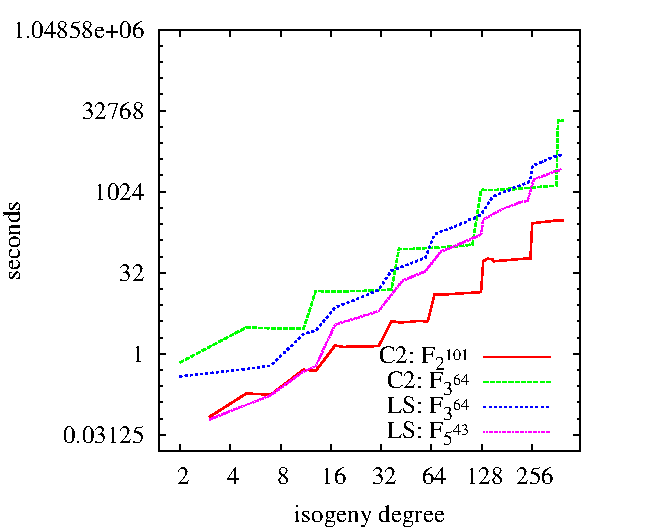
\includegraphics[height=0.5\textwidth]{../isogeny/C2-LS}
    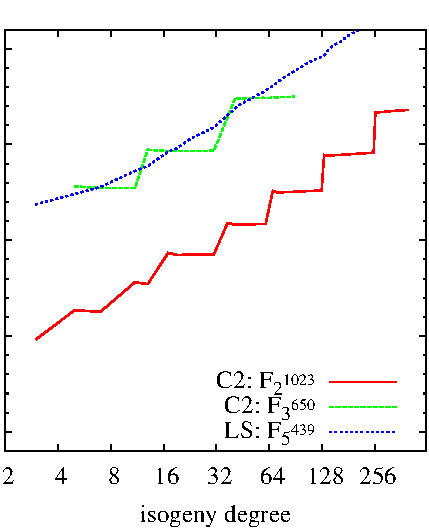
\includegraphics[height=0.5\textwidth]{../isogeny/C2-LS2}
    \caption{Comparative timings for \cite{couveignes96} (C2) and
      \cite{lercier+sirvent08} (LS) over various curves. Plot in
      logarithmic scale.}
  \label{fig:comp}
\end{figure}
\end{frame}

%%
%%

\section{Finite field arithmetic}

\begin{frame}
  \frametitle{The field of definition of $E[p^k]$}
  
  \begin{columns}
    \begin{column}{0.3\textwidth}
      \large\[\xymatrix@C=20pt{
        *[r]{\U_k} \ar@{-}[d]^p & E[p^k] \ar@{-->}[l]\\
        *[r]{\U_{k-1}} \ar@{--}[dd] & E[p^{k-1}] \ar@{-->}[l]\\
        \\
        *[r]{\U_2} \ar@{-}[d]^p & E[p^2] \ar@{-->}[l]\\
        *[r]{\U_1} \ar@{-}[d] & E[p] \ar@{-->}[l]\\
        *[r]{\F_q}
      }\]
    \end{column}
    \begin{column}{0.65\textwidth}
      \begin{center}
        \begin{tikzpicture}[node distance=4em]
          \node(C){$C$}; 
          \node(E)[below of=C]{$E$};
          \node(sqE)[left of=E]{$\widetilde{E}$};
          \scriptsize
          \textcolor<4>{red}{\path[->] (E) edge node[auto,swap]{$\simeq$} (C);}
          \textcolor<3>{red}{\path[->] (C) edge[bend right] (sqE);}
          \textcolor<2>{red}{\path[->] (sqE) edge[bend left] node[auto]{$\frobisog$} (E);}
          \path[->] (E) edge[dashed, bend left]  node[auto]{$V$} (sqE);
        \end{tikzpicture}
      \end{center}
      \begin{block}{$p$-descent (\cite{voloch90})}
        If $\;P_i=(x_i,y_i)\;$ generates $\;E[p^i]$, the solution to
        \begin{equation*}
          \begin{cases}
            \alert<3>{Z^p - Z} &\alert<3>{- \frac{\sqrt[p]{y_i\beta_E(x_i)}}{\sqrt[p-1]{H_E}}}\\
            \alert<2>{X^p} &\alert<2>{- x_i}\\
            \alert<2>{Y^p} &\alert<2>{- y_i}
          \end{cases}
        \end{equation*}
        generates $\;C[p^{i+1}]$.\\
        \alert<4>{Then apply the isomorphism $\;C\isom E$}.
      \end{block}
    \end{column}
  \end{columns}
\end{frame}

%%

\begin{frame}
  \frametitle{Artin-Schreier towers}

  \begin{columns}
    \begin{column}{0.3\textwidth}
      \Large\[\xymatrix{
        *+[r]{\U_k = \frac{\U_{k-1}[X_k]}{X_k^p-X_k-\alpha_{k-1}}}\ar@{-}[d]^p\\
        *+[r]{\U_{k-1}} \ar@{--}[dd]\\
        \\
        *+[r]{\U_{1} = \frac{\U_0[X_1]}{X_1^p-X_1-\alpha_0}} \ar@{-}[d]^p\\
        *+[r]{\U_{0} = \F_q = \frac{\F_p[X_0]}{Q(X_0)}}
      }\]
    \end{column}
    \begin{column}{0.65\textwidth}
      \begin{block}{Artin-Schreier polynomials}
        Artin-Schreier polynomial: 
        \begin{center}
          \emph{\large$X^p - X - \alpha\qquad$} with $\alpha\in\K$
        \end{center}
      \end{block}
      
      \begin{block}{Proposition}
        $X^p-X-\alpha\;$ is either irreducible or split in $\;\K$.
      \end{block}

      \begin{block}{Artin-Schreier extensions}
        Defined by an irreducible Artin-Schreier polynomial
        \begin{center}
          \large\emph{$\LK = \K[X]/(X^p - X - \alpha)$}
        \end{center}
        \alert{ANY} separable extension of degree $p$ can be expressed
        this way.
      \end{block}
    \end{column}
  \end{columns}
\end{frame}

%%

\begin{frame}
  \frametitle{Arithmetic in towers of field extensions}
  
  Special case of arithmetic in $\F_p[X_0,\ldots,X_k]$ modulo a
  \emph{triangular ideal}.
  
  \begin{equation*}
    \F_p[X_0,\ldots,X_k] / \left\{
      \begin{aligned}
        T_k(X_k,\ldots, &X_0)\\
        &\vdots\\
        T_1(X_1, &X_0)\\
        T_0(&X_0)
      \end{aligned}
    \right.
  \end{equation*}

  \begin{overlayarea}{\textwidth}{0.5\textheight}
    \begin{onlyenv}<1>
      \begin{block}{Naive approach}
        \begin{itemize}
        \item Let $\delta=\prod_i\deg_{X_i}T_i$, elements are represented
          using at most $\delta$ monomials;
        \item Plain multiplication yields a multivariate polynomial having
          at most $2^{k+1}\delta$ monomials;
        \item \alert{Any strategy} that multiplies and then reduces modulo
          the ideal has an extra factor of at least \alert{$2^{k+1}$}.
        \item Exponentiation, Inversion, GCD, all depend upon $\;\Mult(\U_k)$,
        \end{itemize}
      \end{block}
    \end{onlyenv}
    
    \begin{onlyenv}<2>
      \begin{block}{Strategies}
        \begin{itemize}
        \item Kronecker substitution \parencite{li+moreno+schost07}\hfill\emph{$\tildO(4^k\delta)$}
        \item Homotopic deformation\\ \parencite{bostan+chowdhury+hoeven+schost}\hfill\emph{$\tildO(\delta)$}
        \item Find a primitive element and change to an univariate
          representation \parencite{alonso+becker+roy+wormann,rouiller99}
          \begin{itemize}
          \item Using fast modular composition \parencite{kedlaya+umans08}\hfill\emph{$O(\delta^{1+o(1)})$}
          \item Specific to Artin-Schreier towers \parencite{df+schost09}\hfill\emph{$\tildO(\delta)$}
          \end{itemize}
        \end{itemize}
      \end{block}
    \end{onlyenv}
  \end{overlayarea}
\end{frame}

%%

\begin{frame}
  \frametitle{One fast tower, many fast towers!}
  
  \begin{center}
    A Fast A-S tower

    \smallskip

    \large$\xymatrix{
      \only<2->{E[p^k]\ar@{-->}[r]} & \only<2->{\U_k \ar@{-}[d]\ar[r]}      & \LK_k \ar@{-}[d]      & \only<2->{\U_k' \ar@{-}[d]\ar[l]}& \only<2->{E'[p^k]\ar@{-->}[l]}\\
      &\only<2->{\U_{k-1} \ar@{--}[dd]\ar[r]} & \LK_{k-1} \ar@{--}[dd] & \only<2->{\U_{k-1}' \ar@{--}[dd]\ar[l]}\\
      \\
      &\only<2->{\U_1 \ar@{-}[dr]\ar[r]}     & \LK_1 \ar@{-}[d]      & \only<2->{\U_1' \ar@{-}[dl]\ar[l]}\\
      &                    &\LK_0
    }$
  \end{center}

  \uncover<2->{ \emph{Theorem (\cite{couveignes00}):} There exist an
    isomorphism algorithm that runs in \alert{$O(k^3\Mult(\LK_k))$}
    operations in $\LK_0$. (Remember that \alert{$\;k=\log_p\card{\LK_k}$})}
\end{frame}

%%

\begin{frame}
  \frametitle{A fast tower}

  \begin{tikzpicture}
    \begin{scope} 
      \only<2>{\color{gray}}
      \draw (0,0) node {\Large$\xymatrix{
          *+[r]{\LK_k = \frac{\LK_{k-1}[X_k]}{X_k^p-X_k-\alpha_{k-1}}}\ar@{-}[d]^p\\
          *+[r]{\LK_{k-1}} \ar@{--}[d]\\
          *+[r]{\LK_1 = \frac{\LK_0[X_1]}{X_1^p-X_1-\alpha_0}} \ar@{-}[d]^p\\
          *+[r]{\LK_0 = \F_q = \frac{\F_p[X_0]}{Q(X_0)}} \ar@{-}[d]^d\\
          *+[r]{\F_p}
        }$};
    \end{scope}

    \begin{scope}[xshift=1.8cm]
      \draw (2,1.5) node {\parbox{3.3cm}{\emph{Idea:} we choose the
          \emph{simplest} tower such that the image of $X_i$ in
          $\LK_i$ is \alert{$\F_p$-primitive}}};
      %
      \uncover<2->{\draw[<->] (0.4,0.5) -- (4,0.5);}
      % 
      \uncover<2->{\draw (2,-0.5) node {\parbox{3.3cm}{and we give fast
            algorithms for the change of basis.}};}
    \end{scope}
      
    \begin{uncoverenv}<2->
      \color{gray}
      \begin{scope}[xshift=8cm]
        \draw (0,0) node {\Large$\xymatrix{
            *+[r]{\LK_k = \frac{\F_p[X_k]}{Q_k(X_k)}}\ar@{-}[d]^p\\
            *+[r]{\LK_{k-1}} \ar@{--}[d]\\
            *+[r]{\LK_1 = \frac{\F_p[X_1]}{Q_1(X_1)}} \ar@{-}[d]^p\\
            *+[r]{\LK_0 = \F_q = \frac{\F_p[X_0]}{Q(X_0)}} \ar@{-}[d]^d\\
            *+[r]{\F_p}
          }$};
      \end{scope}
    \end{uncoverenv}
  \end{tikzpicture}
\end{frame}

%%

\begin{frame}
  \frametitle{Implementations}

  \begin{itemize}
    \setlength{\itemsep}{\baselineskip}
  \item \emph{FAAST} (Fast Arithmetic in Artin-Schreier towers):
    \texttt{C++} with NTL implementation ($\sim6000$ lines) released
    under GPL:
    \hfill\emph{\url{http://www.lix.polytechnique.fr/~defeo/FAAST/}}\hfill\strut
  \item \texttt{C++} benchmarks of Couveignes' algorithm, built on top
    of FAAST.
  \item Including FAAST and algorithms for isogenies in Sage.
  \end{itemize}
\end{frame}

%%

\begin{frame}
  \frametitle{Implementations}
  
  \begin{figure}
    \centering
    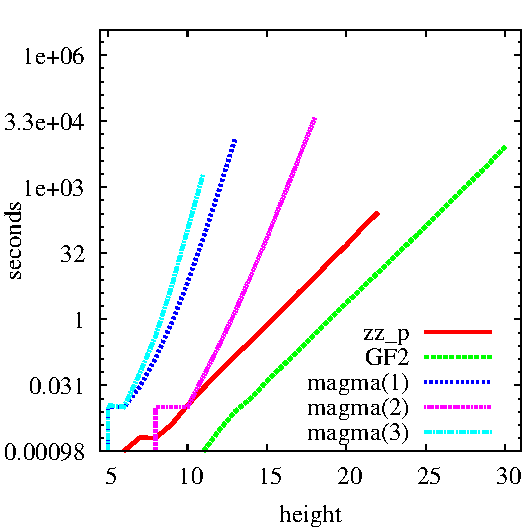
\includegraphics[height=0.5\textwidth]{../artin/build1}
    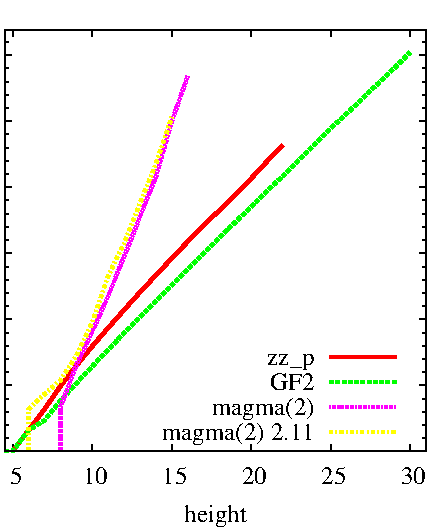
\includegraphics[height=0.5\textwidth]{../artin/iso1}
    
    \caption{Build time (left) and isomorphism time (right) with respect to tower height. Plot is in logarithmic scale.}
    \label{fig:height}
  \end{figure}
\end{frame}

%%

\begin{frame}
  \frametitle{Implementations}

  \begin{figure}
    \centering
    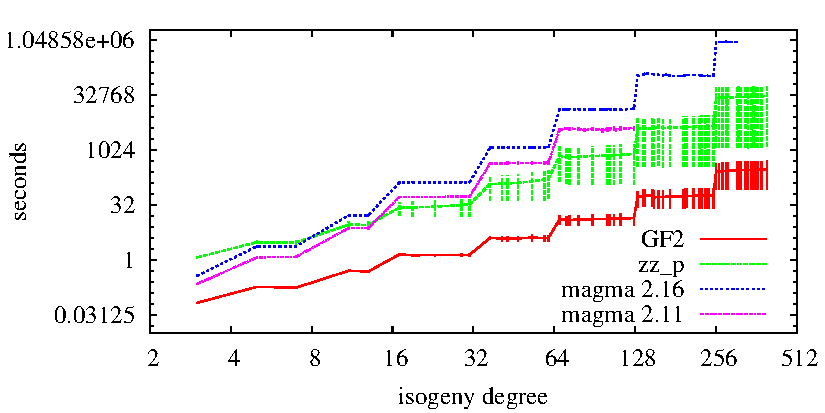
\includegraphics[width=\textwidth]{../isogeny/p2}
    \caption{Comparative timings for different implementations of
      Couveignes' algorithm with curves defined over
      $\F_{2^{101}}$. Plot in logarithmic scale.}
    \label{fig:2-101}
  \end{figure}
\end{frame}

%% 
%%

\section{New uses of optimal Artin-Schreier towers}

\begin{frame}
  \frametitle{Fast Frobenius morphisms}
  
  Let $\sigma : x \mapsto x^{p^d}$ be the Frobenius of $\LK_k/\LK_0$

  \[\xymatrix{
    \LK_k & v^{\sigma^j}\ar@/_/[d]\\
    \LK_{k-1}[x_i] & v^{\sigma^j} = (v_0 + v_1x_i + \cdots + v_{p-1}x_i^{p-1})^{\sigma^j}\ar@{-->}@/_/[dd]\only<2->{\ar@/_/[u]}\\
    \vdots & \\
    \LK_0[x_1,\ldots,x_i] & (v_0 + v_1x_1 + \cdots)^{\sigma^j} = v_0 + v_1x_1^{\sigma^j} + \cdots\only<2->{\ar@{-->}@/_/[uu]}
  }\]

  \uncover<2>{\emph{Complexity:} $\tildO(p^k)$}
\end{frame}

\begin{frame}
  \frametitle{Fast Artin-Schreier vs Normal bases}

  \begin{block}{Fast normal bases for the extension $\F_{q^m}/\F_q$}
    Normal bases allow fast computation of the Frobenius
    morphism. \emph{Fast multiplication} in such bases is an active
    research field.
    \begin{itemize}
    \item Low complexity normal bases\hfill\emph{$O(m^2)$}
    \item Gauss periods \parencite{gao+gathen+panario+shoup00}\hfill\emph{$\tildO(m)$}
    \item Elliptic bases \parencite{couveignes_lercier09}\hfill\emph{$\tildO(m)$}
    \end{itemize}
    Each of the above has limitations and requires a search for
    feasible parameters $(q,m)$.
  \end{block}

  \begin{block}{Fast Frobenius using Artin-Schreier towers}
    Restricted to $m=p^k$, but:
    \begin{itemize}
    \item \emph{Efficiency:} quasi-optimal and fast in practice;
    \item \emph{Instantaneous:} very limited precomputations, no search;
    \item \emph{Scalability:} infinite family of parameters \emph{$(q,p^k)$ for any $k$};
    \item Especially interesting for coding theory: \emph{$(2,2^k)$}.
    \end{itemize}
  \end{block}
\end{frame}

%%

\begin{frame}
  \frametitle{Example: rank-metric decoding of Gabidulin codes}
  
  A length $n$ codeword on the alphabet $\F_{q^m}$ can be represented
  as an $m\times n$ matrix with coefficients in $\F_q$.

  \begin{block}{Hamming distance}
    The \emph{Hamming distance} on $\F_{q^m}$ is very good at correcting errors
    arranged in columns
    \begin{equation*}
      \begin{pmatrix}
        1 & 0 & 1 \\
        0 & 0 & 1 \\
        1 & 1 & 0 \\
        0 & 1 & 1
      \end{pmatrix}
      +
      \begin{pmatrix}
        1 & 0 & 0\\
        0 & 0 & 0\\
        1 & 0 & 0\\
        1 & 0 & 0
      \end{pmatrix}
    \end{equation*}
  \end{block}

  \begin{block}{Rank distance}
    The \emph{rank distance} of two codewords $a,b$ is
    $\text{rank}(a-b)$. It is very good at correcting errors arranged
    in columns \alert{and} rows
    \begin{equation*}
      \begin{pmatrix}
        1 & 0 & 1 \\
        0 & 0 & 1 \\
        1 & 1 & 0 \\
        0 & 1 & 1
      \end{pmatrix}
      +
      \begin{pmatrix}
        1 & 1 & 1\\
        0 & 0 & 0\\
        1 & 1 & 1\\
        1 & 1 & 1
      \end{pmatrix}
    \end{equation*}
  \end{block}
\end{frame}

%%

\begin{frame}
  \frametitle{Gabidulin codes}
  
  \begin{block}{MRD codes}
    For any $(n,k)$-linear code, the rank distance satisfies
    \[d \le n-k+1\]
    Codes that reach this bound are called \emph{MRD} codes.
  \end{block}

  \begin{block}{Gabidulin codes}
    Let \alert{$\;[i] \equiv q^i$}, a \emph{linearized polynomial} is
    one of the form
    \[L_f = f_0 X + f_1 X^{[1]} + \cdots + f_{k-1} X^{[k-1]}.\]
    
    An \emph{$(n,k)$-Gabidulin code} is
    \[C \quad=\quad \left\{(L_f(\alpha_0), \ldots, L_f(\alpha_{n-1})
      \;\middle|\; \deg_\sigma L_f < k\right\} \quad\subset\quad F_{q^m}^n.\]

    Gabidulin codes are MRD. They are the rank-distance equivalent of
    Reed-Solomon codes.
  \end{block}
\end{frame}

%%

\begin{frame}
  \frametitle{Decoding of Gabidulin codes}
  
  \begin{block}{Symbolic product}
    Given two linearized polynomials $L_f,L_g$, their \emph{symbolic
      product} (or \emph{skew product}) is
    \[L_f \otimes L_g = L_f(L_g)\] 

    When $L_f,L_g$ have coefficients in $\F_q$, this is equivalent to
    the ordinary product.
  \end{block}

  \begin{block}{\cite{wachter+afanassiev+sidorenko11}}
    \begin{itemize}
    \item Gabidulin codes can be decoding using the \emph{linearized
        equivalent of the extended Euclidean algorithm};
    \item The complexity of the algorithm is \alert{$O(S(m)\log m)$},
      where $S(m)$ is the cost of performing symbolic product modulo
      $X^{[m]}-X$.
    \item Using \emph{low-complexity normal bases}, \alert{$S(m) = O(m^3)$}.
    \end{itemize}
  \end{block}
\end{frame}

%%

\begin{frame}
  \frametitle{Fast symbolic product using low-complexity normal bases}
  
  \begin{block}{$q$-transforms}
    \begin{itemize}
    \item Let $\beta$ be $\F_q$-normal. The \emph{$q$-transform} of
      $L_f$ w.r.t. $\beta$ is
      \[\left(L_f(\beta^{[0]}), \ldots, L_f(\beta^{[m-1]})\right);\]
    \item If $\tilde{\beta}$ is the dual normal element to $\beta$,
      the \emph{$q$-transform} w.r.t. $\tilde{\beta}$ is the
      \emph{inverse $q$-transform} w.r.t. $\beta$.
    \end{itemize}
  \end{block}

  \begin{block}{Evaluation-Interpolation strategy}
    \begin{itemize}
    \item Compute $(G_0,\ldots,G_{m-1})$, the \emph{$q$-transform} of $L_g$;\hfill\alert{$O(m^3)$}
    \item Compute $H=\left(L_f(G_0), \ldots, L_f(G_{m-1})\right)$;\hfill\alert{$O(m^3)$}
    \item Compute the \emph{inverse $q$-transform} of $H$.\hfill\alert{$O(m^3)$}
    \end{itemize}
  \end{block}
\end{frame}

%%

\begin{frame}
  \frametitle{Faster symbolic product using Artin-Schreier towers}

  \begin{block}{Key observations}
    \begin{itemize}
    \item The $q$-transform is an \alert{ordinary modular product of polynomials};
    \item An $\F_q$-normal element is available for free in our
      Artin-Schreier construction;
    \item Computing the whole normal basis only costs \alert{$\tildO(m\Mult(m))$}.
    \end{itemize}
  \end{block}

  \begin{block}{Evaluation-Interpolation strategy}
    \begin{itemize}
    \item Compute $(G_0,\ldots,G_{m-1})$, the \emph{$q$-transform} of $L_g$;\hfill\alert{$O(\Mult(m^2))$}
    \item Compute $H=\left(L_f(G_0), \ldots, L_f(G_{m-1})\right)$;\hfill\alert{$O(m^\omega)$}
    \item Compute the \emph{inverse $q$-transform} of $H$.\hfill\alert{$O(\Mult(m^2))$}
    \end{itemize}
  \end{block}

  \begin{block}{Remarks}
    \begin{itemize}
    \item Not yet practical, because \alert{$m^\omega$} is in practice
      very close to \alert{$m^3$};
    \item Similar complexities can be obtained using elliptic bases (and
      probably Gauss periods too).
    \end{itemize}
  \end{block}
\end{frame}

%%

\begin{frame}
  \frametitle{Conclusion}
  
  \begin{block}{Summarizing}
    \begin{itemize}
      \setlength{\itemsep}{\baselineskip}
    \item \emph{We have improved Couveignes' algorithm and given its
        first efficient implementation}; it does not beat other
      algorithms for the same task, but it has some interesting
      features that may turn out to be practical.
    \item To reach our goal, \emph{we have given a non-trivial,
        quasi-optimal and practical construction for fast finite
        field arithmetic in some towers which are interesting
        \textit{per-se}}.
    \item This new construction \emph{compares positively with normal
        bases}, although it only covers a very specific case. It has
      interesting \emph{applications in coding theory and network
        coding}.
    \end{itemize}
  \end{block}
\end{frame}


\begin{frame}
  \frametitle{Conclusion}
  
  \begin{block}{The future}
    \begin{itemize}
      \setlength{\itemsep}{\baselineskip}
    \item Improve algorithms for isogenies and modular polynomials,
      possible applications to point-counting in medium and large
      size.
    \item Generalize algorithms to higher genus. Couveignes'
      algorithms are the most promising for genus $2$.
    \item Extend constructions on finite fields, find applications.
    \item Implement, implement, implement!
    \end{itemize}
  \end{block}
\end{frame}

% {\setbeamertemplate{navigation symbols}{}
% \begin{frame}[allowframebreaks]
%   \frametitle{References}
  
%   \printbibliography
% \end{frame}
% }

\end{document}


% Local Variables:
% mode:flyspell
% ispell-local-dictionary:"american"
% mode:TeX-PDF
% mode:reftex
% End:
%
% LocalWords:  Isogeny abelian isogenies hyperelliptic supersingular Frobenius
% LocalWords:  isogenous
